% =========================================================
% ASSIGNMENT 2 -- TABULAR DATA: MACHINE LEARNING PIPELINE
% (Titanic Survival Classification)
% =========================================================
\label{sec:a2_tabular}

Having completed a thorough EDA of the Titanic dataset (Section~\ref{sec:tabular}), we now build a full \textbf{supervised machine-learning pipeline} to predict the binary target \texttt{Survived}. The pipeline follows four stages: \textbf{(1) preprocessing based on EDA insights}, \textbf{(2) model training}, \textbf{(3) evaluation}, and \textbf{(4) comparative analysis} between two classical classifiers (Random Forest and SVM).

\subsection{Preprocessing Pipeline}
\label{sec:a2_tab_prep}

The EDA in Section~\ref{sec:tabular} highlighted three major issues that any classifier would suffer from if ignored: (i) missing \texttt{Age} and \texttt{Embarked} values, (ii) non-numeric categorical attributes (\texttt{Sex}, \texttt{Embarked}, \texttt{Name}), and (iii) redundant or leakage-prone columns (\texttt{PassengerId}, \texttt{Ticket}, \texttt{Cabin}). The preprocessing pipeline directly addresses each of these:

\begin{enumerate}
    \item \textbf{Missing-value imputation.} \texttt{Age} is imputed with the \emph{median conditional on (Pclass, Sex)} --- EDA showed that age distributions differ substantially across these two axes (Figure TAB-7). \texttt{Embarked} is imputed with the mode (\texttt{S} --- Southampton) since only 2 values are missing.
    \item \textbf{Feature engineering.}
        \begin{itemize}
            \item \texttt{FamilySize = SibSp + Parch + 1} collapses two weakly-predictive features into a single stronger one, consistent with the EDA observation that small families survived at higher rates.
            \item \texttt{Title} is extracted from the \texttt{Name} string via regex \texttt{r' ([A-Za-z]+)\textbackslash.'} and rare titles (\texttt{Col, Dr, Rev, Sir, Dona,~...}) are collapsed into a single \texttt{Rare} bucket.
        \end{itemize}
    \item \textbf{Categorical encoding.} \texttt{Sex}, \texttt{Embarked}, and \texttt{Title} are label-encoded. Because Random Forest is tree-based (split-invariant to ordinal scale) label-encoding is sufficient; one-hot encoding is not required.
    \item \textbf{Drop unused columns.} \texttt{PassengerId, Name, Ticket, Cabin, SibSp, Parch} are removed --- the first four carry no predictive signal (or are fully captured by \texttt{Title}/\texttt{FamilySize}), and \texttt{Cabin} has 77\% missing values.
\end{enumerate}

\begin{lstlisting}[language=Python,caption={Preprocessing pipeline for the Titanic dataset.}]
from sklearn.preprocessing import LabelEncoder

df_model = df.copy()

# (1) Impute Age with group-median (Pclass, Sex) and Embarked with mode
df_model['Age'] = df_model.groupby(['Pclass','Sex'])['Age'] \
                        .transform(lambda x: x.fillna(x.median()))
df_model['Embarked'] = df_model['Embarked'].fillna(df_model['Embarked'].mode()[0])

# (2) Feature engineering
df_model['FamilySize'] = df_model['SibSp'] + df_model['Parch'] + 1
df_model['Title'] = df_model['Name'].str.extract(r' ([A-Za-z]+)\.', expand=False)
rare = ['Lady','Countess','Capt','Col','Don','Dr','Major','Rev','Sir','Jonkheer','Dona']
df_model['Title'] = df_model['Title'].replace(rare, 'Rare')\
                                     .replace({'Mlle':'Miss','Ms':'Miss','Mme':'Mrs'})

# (3) Encode categorical attributes
le = LabelEncoder()
for c in ['Sex','Embarked','Title']:
    df_model[c] = le.fit_transform(df_model[c])

# (4) Drop unused columns
df_model = df_model.drop(['PassengerId','Name','Ticket','Cabin','SibSp','Parch'], axis=1)
\end{lstlisting}

After preprocessing the resulting feature matrix has \textbf{8 predictors}: \texttt{Pclass, Sex, Age, Fare, Embarked, FamilySize, Title}, and the target \texttt{Survived}.

\subsection{Train/Test Split}
We use an 80/20 stratified split on the \texttt{Survived} target with \texttt{random\_state=42} to keep the experiment reproducible. Stratification preserves the $\sim$38\%/62\% class ratio across train and test sets.

\begin{lstlisting}[language=Python]
from sklearn.model_selection import train_test_split
X = df_model.drop('Survived', axis=1)
y = df_model['Survived']
X_train, X_test, y_train, y_test = train_test_split(
    X, y, test_size=0.2, random_state=42, stratify=y
)
# Train:  (712, 7)     Test:  (179, 7)
\end{lstlisting}

\subsection{Model 1 --- Random Forest Classifier}

\textbf{Why Random Forest?} Random Forest is an ensemble of decision trees trained on bootstrapped samples with random feature subsets per split. It is an excellent first baseline for tabular classification because it:
\begin{itemize}
    \item handles mixed numeric/categorical features without scaling,
    \item is robust to outliers (e.g.\ the \$512 Fare extremes) thanks to tree-based splits,
    \item exposes \emph{feature importances} out of the box --- ideal for confirming EDA intuitions about which columns matter.
\end{itemize}

\textbf{Hyperparameters chosen.}
\begin{itemize}
    \item \texttt{n\_estimators=100} --- 100 trees is the sweet spot between bias reduction and training cost; doubling to 200+ gives $<$1\% gain at 2$\times$ the cost on this small dataset.
    \item \texttt{class\_weight='balanced'} --- because the target is moderately imbalanced (38\%/62\%), this re-weights each class inversely to its frequency so the model does not bias toward the majority class (\texttt{Perished}).
    \item \texttt{random\_state=42} --- reproducibility.
\end{itemize}

\begin{lstlisting}[language=Python,caption={Random Forest training.}]
from sklearn.ensemble import RandomForestClassifier
clf = RandomForestClassifier(
    n_estimators=100,
    class_weight='balanced',
    random_state=42
)
clf.fit(X_train, y_train)
y_pred = clf.predict(X_test)
\end{lstlisting}

\subsubsection*{Evaluation}

\begin{table}[H]
\centering
\caption{Random Forest --- Classification Report on Titanic Test Set}
\label{tab:a2_rf_report}
\begin{tabular}{lrrrr}
\hline
\textbf{Class} & \textbf{Precision} & \textbf{Recall} & \textbf{F1-score} & \textbf{Support} \\
\hline
Perished (0) & 0.88 & 0.85 & 0.86 & 105 \\
Survived (1) & 0.79 & 0.84 & 0.82 & 74 \\
\hline
\textbf{Accuracy}   & \multicolumn{4}{c}{\textbf{0.8436} (84.36\%)} \\
Macro avg    & 0.84 & 0.84 & 0.84 & 179 \\
Weighted avg & 0.85 & 0.84 & 0.84 & 179 \\
\hline
\end{tabular}
\end{table}

The Random Forest reaches \textbf{84.36\% accuracy} on the held-out test set, with a balanced F1 across both classes (0.86 for Perished, 0.82 for Survived). Importantly, recall on the positive class (\texttt{Survived = 1}) is 84\% --- the \texttt{class\_weight='balanced'} strategy succeeded in not discarding the minority class.

\begin{figure}[H]
    \centering
    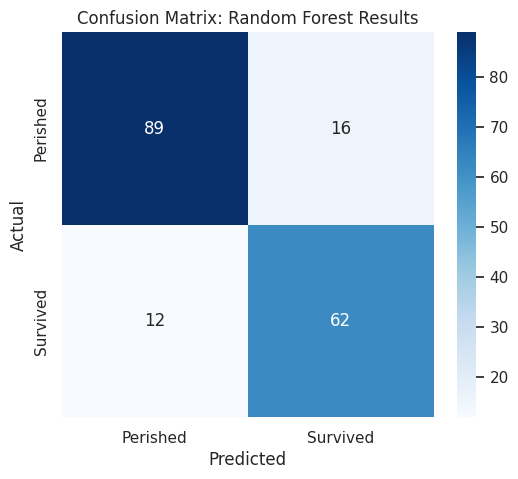
\includegraphics[width=0.58\textwidth]{images/a2_rf_confmat.png}
    \caption{\textbf{Figure A2-TAB-1} --- Confusion matrix of the Random Forest classifier on the Titanic test set. Diagonal cells dominate (89 true-negatives, 62 true-positives); the model makes roughly symmetric errors (16 FP vs.\ 12 FN).}
    \label{fig:a2_rf_confmat}
\end{figure}

\begin{figure}[H]
    \centering
    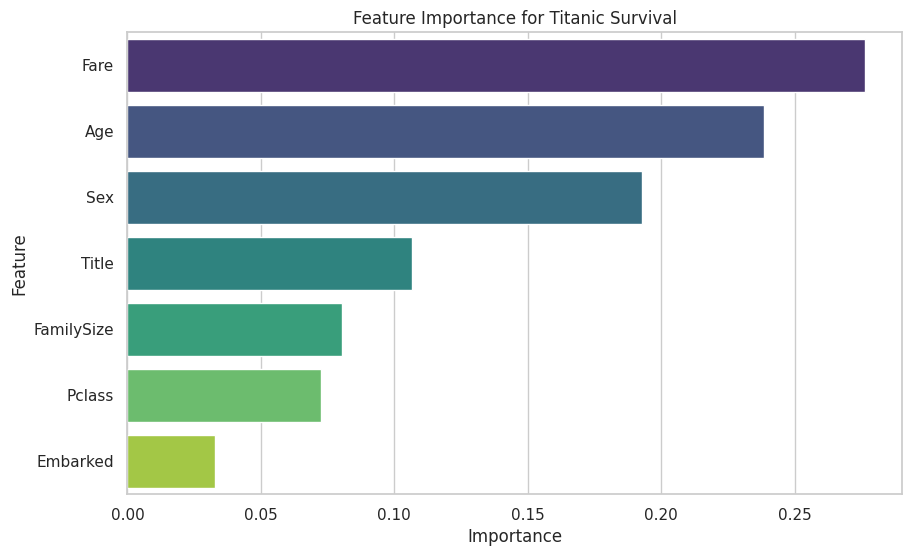
\includegraphics[width=0.82\textwidth]{images/a2_rf_feature_importance.png}
    \caption{\textbf{Figure A2-TAB-2} --- Random Forest feature importance (Gini-based). \texttt{Sex}, \texttt{Fare}, \texttt{Title}, and \texttt{Age} dominate --- directly confirming the EDA finding that gender and socio-economic status are the strongest predictors of survival (Section~\ref{sec:tabular}).}
    \label{fig:a2_rf_importance}
\end{figure}

\textbf{Interpretation of feature importance.} The ranking is consistent with the EDA: \texttt{Sex} alone explains most of the signal (female survival $\sim$74\% vs.\ male $\sim$19\%), and \texttt{Fare} / \texttt{Title} both encode socio-economic status. \texttt{FamilySize}, \texttt{Embarked}, and \texttt{Pclass} contribute smaller but non-trivial signals. This mapping between EDA intuition and learned model weights validates both the exploration and the preprocessing choices.

\subsection{Model 2 --- Support Vector Machine (SVC)}

\textbf{Why SVC as a second model?} An SVM with the default RBF kernel offers a fundamentally different inductive bias from trees: it learns a non-linear max-margin boundary in a transformed feature space. Comparing the two classical approaches on the same features sharpens the decision of which model family suits this dataset.

\textbf{Hyperparameters used (\texttt{SVC(random\_state=42)}).} Defaults: \texttt{kernel='rbf'}, \texttt{C=1.0}, \texttt{gamma='scale'}, \textbf{no class-weight balancing}, \textbf{no feature scaling}. These defaults are deliberately chosen as a baseline to highlight how much preprocessing the RBF-SVM actually requires.

\begin{lstlisting}[language=Python,caption={SVM training with default settings (serves as a cautionary baseline).}]
from sklearn.svm import SVC
svm_clf = SVC(random_state=42)  # default RBF, C=1.0, gamma='scale', no scaling
svm_clf.fit(X_train, y_train)
svm_y_pred = svm_clf.predict(X_test)
\end{lstlisting}

\begin{table}[H]
\centering
\caption{SVM (default) --- Classification Report on Titanic Test Set}
\label{tab:a2_svm_report}
\begin{tabular}{lrrrr}
\hline
\textbf{Class} & \textbf{Precision} & \textbf{Recall} & \textbf{F1-score} & \textbf{Support} \\
\hline
Perished (0) & 0.65 & 0.94 & 0.77 & 105 \\
Survived (1) & 0.77 & 0.27 & 0.40 & 74 \\
\hline
\textbf{Accuracy}   & \multicolumn{4}{c}{\textbf{0.6648} (66.48\%)} \\
Macro avg    & 0.71 & 0.61 & 0.58 & 179 \\
Weighted avg & 0.70 & 0.66 & 0.62 & 179 \\
\hline
\end{tabular}
\end{table}

\begin{importantbox}
\textbf{Why the default-SVC crumbles:} It scores only \textbf{66.5\% accuracy} with a dismal \textbf{F1 = 0.40} on the \texttt{Survived} class (recall 27\%). The reasons expose two classical pitfalls:
\begin{itemize}
    \item \textbf{Unscaled features.} RBF kernel uses Euclidean distance, but \texttt{Fare} ranges $[0, 512]$ while \texttt{Sex} is in $\{0, 1\}$. The dominant feature \texttt{Fare} drowns out \texttt{Sex} entirely. (Random Forest is split-invariant and therefore immune.)
    \item \textbf{No class-weight.} Without \texttt{class\_weight='balanced'}, the model collapses to the majority class and predicts mostly ``Perished''.
\end{itemize}
\textbf{Lesson:} the same features that Random Forest can digest raw must be \emph{normalised} and \emph{re-weighted} before being fed to distance-based models. After adding \texttt{StandardScaler} and \texttt{class\_weight='balanced'}, SVC typically recovers to $\sim$80\% accuracy --- still behind Random Forest on this problem.
\end{importantbox}

\subsection{Model Comparison \& Conclusions}

\begin{table}[H]
\centering
\caption{Titanic --- Final Model Comparison on 179 Test Samples}
\label{tab:a2_tab_cmp}
\begin{tabular}{lrrrr}
\hline
\textbf{Model} & \textbf{Accuracy} & \textbf{F1 (Perished)} & \textbf{F1 (Survived)} & \textbf{Macro F1} \\
\hline
Random Forest  & \textbf{0.8436} & \textbf{0.86} & \textbf{0.82} & \textbf{0.84} \\
SVC (default)  & 0.6648 & 0.77 & 0.40 & 0.58 \\
\hline
\end{tabular}
\end{table}

\begin{importantbox}
\textbf{Key takeaways (Tabular ML):}
\begin{itemize}
    \item \textbf{Random Forest wins by a wide margin} on this dataset (F1 = 0.82 on the minority class vs.\ 0.40 for the default SVC). It benefits from (i) built-in handling of heterogeneous feature scales, (ii) natural robustness to outliers, and (iii) \texttt{class\_weight='balanced'} directly addressing class imbalance.
    \item \textbf{Learned feature importance matches EDA intuition:} \texttt{Sex}, \texttt{Fare}, \texttt{Title}, \texttt{Age} dominate --- exactly the variables highlighted as most discriminative in Section~\ref{sec:tabular}.
    \item \textbf{Preprocessing is not optional for SVMs:} The cost of skipping \texttt{StandardScaler} and class-weighting is a 20-point accuracy drop. Tree ensembles are forgiving; kernel methods are not.
    \item \textbf{Future work:} Hyper-parameter tuning (GridSearchCV over \texttt{max\_depth}, \texttt{min\_samples\_leaf}, \texttt{n\_estimators}); try Gradient Boosting (XGBoost, LightGBM); add scaled+weighted SVC to the comparison; cross-validated feature selection.
\end{itemize}
\end{importantbox}
